\documentclass[11pt,a4paper]{article}
\usepackage[utf8]{inputenc}
\usepackage[T1]{fontenc}
\usepackage{lmodern}
\usepackage[french]{babel}
\usepackage{amsmath,amssymb,amsfonts}
\usepackage{geometry}
\geometry{top=2.5cm, bottom=2.5cm, left=2.5cm, right=2.5cm}
\usepackage{graphicx}
\usepackage{booktabs}
\usepackage{tabularx}
\usepackage{xcolor}
\usepackage{microtype}
\usepackage{hyperref}

\hypersetup{
    colorlinks=true,
    linkcolor=blue!70!black,
    citecolor=blue!70!black,
    urlcolor=blue!70!black
}

\title{\textbf{\Large La Lune et l'évacuation du moment cinétique : capture de matière lors d'un survol planétaire rasant prograde}\\
\large Avec une note sur l'apport différé de volatils par le même passage}

\author{\textbf{Michel Debailleul}\\
\small Chercheur indépendant, Belgique\\
\small Géophysicien --- M.Sc., Université libre de Bruxelles (ULB)\\
\small ORCID: \href{https://orcid.org/0009-0003-1222-1433}{0009-0003-1222-1433} \quad | \quad \href{mailto:michel.debailleul@yahoo.fr}{michel.debailleul@yahoo.fr}
}

\date{18 septembre 2026\\[4pt]\footnotesize\textcopyright{} 2026 Michel Debailleul --- \href{https://creativecommons.org/licenses/by-nc/4.0/}{CC BY-NC 4.0}}

\begin{document}

\maketitle

\begin{abstract}
Toute théorie de l'origine lunaire invoquant une proto-Terre en rotation rapide hérite du problème du moment cinétique : la rotation propre d'un tel corps dépasse celle du système Terre--Lune actuel d'environ un facteur deux, et cet excédent doit être évacué. Les mécanismes connus --- capture dans la résonance d'évection solaire ou transition du plan de Laplace --- agissent sur un couple Terre--Lune déjà formé. Cet article examine une voie complémentaire agissant pendant l'événement lui-même. Lorsqu'un corps de masse planétaire frôle une proto-Terre proche de sa limite de rupture rotationnelle, les matériaux superficiels de la bande de basses latitudes sont soulevés, et une fraction bien définie de cette matière s'échappe liée au perturbateur, emportant avec elle son moment cinétique spécifique.

Nous calculons directement cette fraction. Les éléments de la bande de basses latitudes sont libérés en corotation lorsque la résultante verticale de la gravité, de l'accélération centrifuge et du champ différentiel exact du perturbateur s'oriente vers l'extérieur, puis sont intégrés le long de la trajectoire hyperbolique réelle du survol. Sur une grille explorant des masses du perturbateur comprises entre $0{,}5$ et $0{,}95\,M_\oplus$, des distances au périastre de $2{,}8$ à $3{,}5\,R_\oplus$, des inclinaisons de $20$ à $30^\circ$ et deux degrés de dilatation proto-terrestre, et dans les configurations où le soulèvement reste significatif, la fraction capturée est comprise entre $\phi_{\oplus\to B} = 0{,}19$ et $0{,}28$ du matériau soulevé ; un cas limite où seulement $4\,\%$ de la bande est soulevée tombe à $0{,}06$. Le moment cinétique spécifique emporté est de $0{,}93$ à $1{,}00\,\Omega_\oplus R_{\mathrm{eq}}^2$ --- c'est-à-dire essentiellement la valeur équatoriale, soit environ cinq fois la moyenne du corps. Évacuer la totalité de l'excédent, $1{,}07\,L_{\mathrm{EM}}$, exigerait d'emporter $8{,}3\,M_L$. Mais le moment cinétique de la matière soulevée ne peut excéder le spin du corps, ce qui borne le retrait net à environ $0{,}53\,L_{\mathrm{EM}}$ dans la configuration de référence : ce canal couvre au plus environ la moitié de l'excédent, et réduit d'autant ce que doivent accomplir les mécanismes postérieurs à la formation de la Lune. Dans le contrôle rétrograde, rien n'est capturé et l'intégralité de la population soulevée retombe.

Ce même calcul délimite strictement la portée du mécanisme. Le matériau soulevé n'atteint pas lui-même la limite de Roche dès lors que le passage est incliné des $20$ à $25^\circ$ qu'impose le dégagement du disque ; ce canal évacue donc du moment cinétique sans fournir la masse de la Lune. Le vecteur de moment cinétique emporté fait moins de $2^\circ$ avec l'axe de rotation, de sorte que le passage ne compromet pas l'obliquité observée. Enfin, la géométrie du survol qui optimise cette capture amène simultanément le propre lobe de Roche du perturbateur à portée d'une enveloppe volatile dilatée. Dans la théorie proposée, ce débordement alimenterait une traînée de volatils dont la ré-accrétion différée fournirait principalement l'eau terrestre et, dans une moindre mesure, une contribution au réservoir circumterrestre puis à la Lune.
\end{abstract}

\noindent\textbf{Mots-clés :} Système Terre--Lune ; moment cinétique ; survol rasant ; effeuillage par marée ; lobe de Roche ; eau lunaire ; apport des volatils.

\vspace{1em}
\section{Le problème}

Le système Terre--Lune possède aujourd'hui un moment cinétique total $L_{\mathrm{EM}} \approx 3{,}5 \times 10^{34}\,\mathrm{kg\,m^2\,s^{-1}}$. Les scénarios formant la Lune à partir de matière d'origine terrestre requièrent généralement une proto-Terre en rotation proche de sa limite de stabilité, et un tel corps en transporte considérablement plus. Pour une proto-Terre de masse actuelle avec une rotation réduite $\tilde{\omega} = \Omega_\oplus / \sqrt{GM/R_{\mathrm{eq}}^3} = 0{,}97$ et un rayon équatorial $R_{\mathrm{eq}} = 1{,}70\,R_\oplus$, le spin s'écrit :
\begin{equation}
S_\oplus \simeq k_{\mathrm{eff}} M_\oplus \Omega_\oplus R_{\mathrm{eq}}^2 \simeq 2{,}07\,L_{\mathrm{EM}},
\end{equation}
où $k_{\mathrm{eff}} \simeq 0{,}19$ prend en compte un noyau métallique demeuré compact au centre alors que le manteau silicaté est dilaté ; adopter la valeur uniforme $k \simeq 0{,}25$ surévaluerait le spin. L'excédent est d'un facteur deux, et il doit impérativement être évacué.

Le cadre de référence pour l'origine de la Lune repose sur l'impact géant et l'accrétion d'un satellite à partir du disque généré \cite{Canup2023, Ida1997, Salmon2012, Kokubo2000}. Le problème énoncé ici se pose pour toute variante initiée par un rotateur rapide. Deux voies sont établies, toutes deux agissant une fois la Lune formée : la capture dans la résonance d'évection solaire et la transition du plan de Laplace \cite{Murray1999, Tremaine2009, Cuk2012}. Le présent article examine une troisième voie, agissant \emph{pendant} l'événement lui-même, et répond à une question accessible par calcul direct : \emph{combien de moment cinétique un corps planétaire en survol rasant emporte-t-il sous forme de matière ?} Les rencontres non collisionnelles sont d'ailleurs déjà reconnues comme un processus efficace dans la dynamique Terre--Lune primitive \cite{Pahlevan2015}, à un moment ultérieur de l'histoire.

Le mécanisme est élémentaire. Une proto-Terre proche de sa vitesse de rupture n'est maintenue cohérente, dans sa bande de basses latitudes, que par une faible gravité effective résiduelle. La marée différentielle d'un corps planétaire passant à quelques rayons terrestres annule cette cohésion. La matière soulevée provient des régions les plus distantes de l'axe de rotation, emportant un moment cinétique spécifique très élevé, et une fraction de celle-ci termine le survol liée au perturbateur plutôt qu'à la Terre. Le perturbateur s'éloignant sur une trajectoire hyperbolique, cette fraction est définitivement perdue pour le système terrestre.

Deux voies doivent d'abord être écartées explicitement. L'assistance gravitationnelle subie par le perturbateur est élastique dans le référentiel de la proto-Terre : il repart avec la même vitesse relative et seule sa direction change, ce qui échange du moment cinétique héliocentrique (un budget distinct). Par ailleurs, le couple de marée exercé sur la figure de la proto-Terre lors d'un passage unique ne représente que $0{,}02$ à $0{,}12\,L_{\mathrm{EM}}$ pour $k_2/Q$ compris entre $0{,}02$ et $0{,}10$. Aucun de ces effets ne comble le déficit. Parmi les processus agissant pendant ce survol, le transport de matière est le seul canal identifié ici ayant le bon ordre de grandeur, et c'est son efficacité que nous calculons.

\paragraph{Cadre et périmètre de l'étude.} Cet article s'inscrit dans le cadre d'une monographie compagne \cite{Debailleul2026}, dans laquelle un réservoir circumterrestre secondaire préexiste au survol et fournit l'essentiel de la matière lunaire. Le corps de passage agit d'abord comme un agent gravitationnel transitoire qui redistribue la masse et le moment cinétique de ce réservoir et aide une fraction de la matière déjà circumterrestre à franchir la limite de Roche. En parallèle, le même passage favorise le soulèvement de matière superficielle dans la bande de basses latitudes, dont une fraction peut être emportée avec $B$, et il rend disponible une enveloppe volatile de $B$ susceptible d'alimenter ultérieurement le système terrestre. Rien ici ne suppose que la Lune soit fabriquée par arrachement direct de la proto-Terre. La thèse défendue est délimitée : le canal étudié dans cet article évacue une quantité calculable de moment cinétique par emport de matière ; cette quantité est bornée par l'inventaire de moment cinétique du corps et couvre au plus environ la moitié du budget requis.

\section{Méthode}

\subsection{Modèle}
La proto-Terre est modélisée comme un corps à condensation centrale en rotation rigide, doté d'un potentiel effectif $\Phi = -GM/r - \frac{1}{2}\Omega_\oplus^2 \varpi^2$, de sorte que son champ extérieur est monopolaire ($J_2 = 0$) et sa surface est l'équipotentielle de rayon équatorial $R_{\mathrm{eq}}$. Le perturbateur $B$, de masse $\mu_B M_\oplus$, suit la conique hyperbolique exacte du problème des deux corps relatif avec $\mu_{\mathrm{tot}} = G(M_\oplus + M_B)$, périastre $q_B$, argument du périastre $\omega_B = 90^\circ$ et inclinaison $i_B$ mesurée depuis l'équateur de rotation, le périastre se situant ainsi à la latitude $i_B$. L'accélération différentielle subie par une parcelle située en $\mathbf{r}$,
\begin{equation}
\mathbf{a}_{B,\mathrm{diff}} = -G M_B \left[ \frac{\mathbf{r} - \mathbf{r}_B(t)}{|\mathbf{r} - \mathbf{r}_B(t)|^3} + \frac{\mathbf{r}_B(t)}{|\mathbf{r}_B(t)|^3} \right],
\end{equation}
est utilisée sans développement multipolaire, le régime rasant imposant des modules $|\mathbf{r}|$ et $|\mathbf{r}_B|$ comparables.

\subsection{Critère de libération}
Les éléments de surface sont discrétisés en latitude sur la bande de basses latitudes et en longitude, et tournent avec le corps jusqu'à leur libération éventuelle. Un élément est relâché, en corotation, à l'instant où la composante orientée selon la normale extérieure locale de la somme (gravité $+$ force centrifuge $+$ marée) devient positive. Au point sous-perturbateur équatorial, cela se ramène à la condition adimensionnelle :
\begin{equation}
2\,\mu_B \left(\frac{R_{\mathrm{eq}}}{q_B}\right)^3 + \tilde{\omega}^2 \ge 1,
\end{equation}
où le second terme représente la part apportée par la rotation propre du corps et le premier celle fournie par $B$. Aucun des deux ne suffit isolément : une proto-Terre à la rotation critique atteint tout juste l'égalité sans $B$, et $B$ seul n'arrache rien d'un rotateur lent. Pour la configuration de référence, le membre de gauche vaut $1{,}29$, et la zone soulevée s'étend jusqu'à $\pm 26^\circ$ de latitude. Évaluer ce critère à chaque pas de temps est crucial car la zone active se déplace avec la rotation du corps : avec un survol effectif de $5$ à $12\,\mathrm{h}$ face à une période de rotation de $3{,}21\,\mathrm{h}$, la bande passe sous le perturbateur près de deux fois.

\subsection{Intégration et classification}
Les éléments libérés sont intégrés via un schéma de Runge--Kutta d'ordre 4 dans le champ monopolaire terrestre complété par le champ différentiel de $B$, conjointement avec le mouvement de $B$. Un élément qui retombe sous la surface est classé comme ré-accrété. La classification finale s'opère lorsque $B$ s'éloigne au-delà de $8\,q_B$, distance à laquelle son champ différentiel tombe à $0{,}5\,\%$ de l'attraction centrale : un élément est considéré comme \emph{capturé} si son énergie par rapport à $B$ est négative, \emph{échappé} s'il n'est lié à aucun des deux corps, et sinon \emph{lié à la Terre}. Dans ce dernier cas, son rayon de circularisation $r_{\mathrm{circ}} = j^2/GM$ détermine s'il appartient à la région externe au-delà de la limite de Roche $a_R = 2{,}903\,R_\oplus$ ou au disque interne.

\subsection{Configuration de référence et convergence}
\noindent\fbox{
\parbox{0.96\linewidth}{
\textbf{Valeurs adoptées :}\\
$\tilde{\omega} = 0{,}97$, $R_{\mathrm{eq}} = 1{,}70\,R_\oplus$, $\mu_B = 0{,}95$, $q_B = 3{,}0\,R_\oplus$, $\omega_B = 90^\circ$, $v_\infty = 2\,\mathrm{km\,s^{-1}}$, passage prograde, $e_B = 1{,}10$.\\
Période de rotation $3{,}21\,\mathrm{h}$ ; spin $2{,}07\,L_{\mathrm{EM}}$ ; marge de non-contact $7\,\%$ et marge de rupture de marée $9\,\%$ sur $q_B$ pour un perturbateur de densité moyenne $3{,}93\,\mathrm{g\,cm^{-3}}$.
}
}
\vspace{0.5em}

La grille nominale contient $41 \times 240 = 9\,840$ éléments avec un pas temporel de $10\,\mathrm{s}$. Réduire le pas de temps de moitié à deux reprises modifie les résultats de moins de $0{,}5\,\%$ ; raffiner la grille de $21 \times 120$ à $61 \times 360$ modifie les fractions obtenues de moins de $2\,\%$.

\section{Résultats}

\subsection{Devenir de la matière soulevée}
Entre $12$ et $15\,\%$ de la bande quitte la surface, et son destin est nettement tranché : la majeure partie retombe en quelques heures, et environ un quart s'éloigne lié à $B$ (tableau~\ref{tab:fate}).

\begin{table}[h!]
\centering
\caption{Devenir de la matière soulevée, en fractions de la matière soulevée. Calcul en particules-tests, sans autogravité, collisions mutuelles, pression ni hydrodynamique. La dernière ligne correspond au contrôle rétrograde à latitude de périastre identique.}
\vspace{0.5em}
\label{tab:fate}
\setlength{\tabcolsep}{5pt}
\begin{tabular}{lccccc}
\toprule
 & au-delà de $a_R$ & disque interne & retombée & échappée & capturée par $B$ \\
\midrule
$i_B = 0^\circ$ (coplanaire) & $1{,}2\,\%$ & $2{,}5\,\%$ & $68{,}4\,\%$ & $10{,}2\,\%$ & $17{,}7\,\%$ \\
$i_B = 20^\circ$            & $0{,}7\,\%$ & $2{,}2\,\%$ & $69{,}9\,\%$ & $0{,}0\,\%$  & $\mathbf{27{,}2\,\%}$ \\
$i_B = 25^\circ$            & $0{,}0\,\%$ & $2{,}8\,\%$ & $72{,}6\,\%$ & $0{,}0\,\%$  & $\mathbf{24{,}6\,\%}$ \\
$i_B = 30^\circ$            & $0{,}0\,\%$ & $2{,}9\,\%$ & $75{,}2\,\%$ & $0{,}0\,\%$  & $\mathbf{21{,}9\,\%}$ \\
\midrule
rétrograde, $25^\circ$      & $0{,}0\,\%$ & $0{,}0\,\%$ & $100\,\%$  & $0{,}0\,\%$  & $\mathbf{0{,}0\,\%}$ \\
\bottomrule
\end{tabular}
\end{table}

Le contrôle rétrograde est sans ambiguïté : l'intégralité de la population soulevée retombe sur la proto-Terre et absolument rien ne part avec le perturbateur. L'origine de cette asymétrie réside dans la cohérence temporelle. Pour la configuration de référence, la vitesse angulaire de rotation est de $5{,}43 \times 10^{-4}\,\mathrm{rad\,s^{-1}}$ et celle de $B$ au périastre de $4{,}83 \times 10^{-4}$, de sorte qu'en prograde un élément de la bande ne dérive par rapport au perturbateur qu'à $6{,}0 \times 10^{-5}\,\mathrm{rad\,s^{-1}}$ et demeure sous son influence directe tout au long du survol. En rétrograde, la vitesse relative atteint $1{,}03 \times 10^{-3}\,\mathrm{rad\,s^{-1}}$ (dix-sept fois supérieure), et les impulsions alternées s'annulent presque parfaitement.

\subsection{La fraction capturée est robuste}
Pour des masses du perturbateur allant de $0{,}5$ à $0{,}95\,M_\oplus$, des distances d'approche de $2{,}8$ à $3{,}5\,R_\oplus$, des inclinaisons de $20$ à $30^\circ$ et deux degrés de dilatation, et dans les configurations où le soulèvement reste significatif, $\phi_{\oplus\to B}$ reste compris entre $0{,}19$ et $0{,}28$, et entre $0{,}21$ et $0{,}26$ à $i_B = 25^\circ$ (figure~\ref{fig:capture}). La seule exception, $\phi_{\oplus\to B} = 0{,}06$ pour $\mu_B = 0{,}5$ à $q_B = 3{,}5\,R_\oplus$, correspond à la configuration où le soulèvement lui-même devient marginal : seuls $4\,\%$ de la bande quittent alors la surface. Le mécanisme opère comme un processus en deux étapes bien découplées : la géométrie gouverne la masse totale qui quitte la proto-Terre, et une fraction remarquablement constante d'environ un quart de cette matière se retrouve définitivement liée au perturbateur.

\subsection{Le bras de levier équatorial}
Le moment cinétique spécifique moyen (pondéré par la masse) de la population capturée est de $0{,}97\,\Omega_\oplus R_{\mathrm{eq}}^2$ pour la configuration de référence, et reste compris entre $0{,}93$ et $1{,}00$ sur toute la grille. Une estimation courante attribue à la matière perdue le moment spécifique moyen du corps, $k_{\mathrm{eff}}\Omega_\oplus R_{\mathrm{eq}}^2$ ; le calcul montre qu'en réalité la matière soulevée puis capturée emporte $1/k_{\mathrm{eff}} \simeq 5$ fois cette valeur, car elle provient des basses latitudes, où le bras de levier par rapport à l'axe de rotation reste proche de sa valeur équatoriale. La population soulevée dans son ensemble porte en moyenne $\langle j_z\rangle_{\mathrm{lift}} = 0{,}928\,\Omega_\oplus R_{\mathrm{eq}}^2$, contre $\langle j_z\rangle_{\mathrm{cap}} = 0{,}966\,\Omega_\oplus R_{\mathrm{eq}}^2$ pour la matière capturée : la capture est donc légèrement biaisée, d'environ $4\,\%$, vers les plus grands moments spécifiques.

\begin{figure}[htbp]
\centering
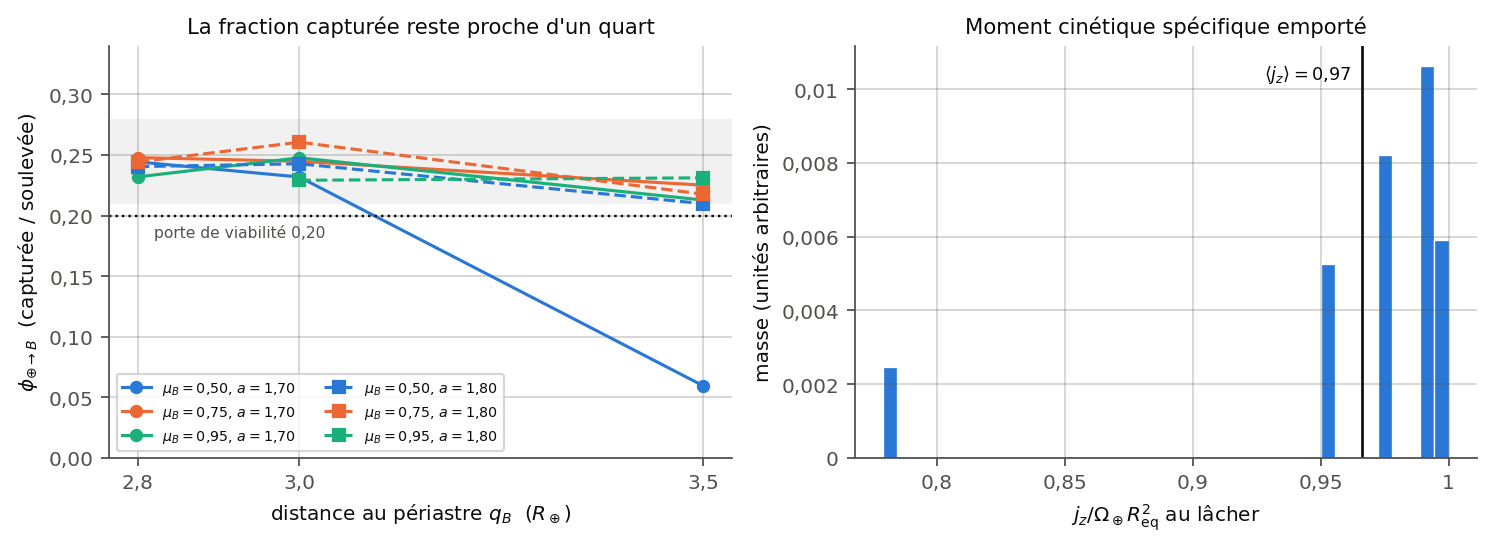
\includegraphics[width=\textwidth]{fig_capture_fr.png}
\caption{À gauche : fraction capturée $\phi_{\oplus\to B}$ sur la grille de paramètres, à $i_B=25^\circ$ ; traits pleins et cercles pour $R_{\mathrm{eq}}=1{,}70\,R_\oplus$, tirets et carrés pour $1{,}80\,R_\oplus$. La bande grisée marque l'intervalle $0{,}21$--$0{,}28$. L'unique point bas correspond à la configuration où le soulèvement lui-même devient marginal. À droite : distribution pondérée par la masse du moment cinétique spécifique emporté, en unités de $\Omega_\oplus R_{\mathrm{eq}}^2$, pour la configuration de référence à $i_B=25^\circ$.}
\label{fig:capture}
\end{figure}

\section{Le budget de moment cinétique}

\noindent\fbox{
\parbox{0.96\linewidth}{
\textbf{Ce qu'exigerait une fermeture complète :}\\
Avec $\langle j_z \rangle_{\mathrm{cap}} = 0{,}97\,\Omega_\oplus R_{\mathrm{eq}}^2 = 6{,}2 \times 10^{10}\,\mathrm{m^2\,s^{-1}}$, évacuer $\Delta L = 1{,}07\,L_{\mathrm{EM}} = 3{,}7 \times 10^{34}\,\mathrm{kg\,m^2\,s^{-1}}$ imposerait d'emporter
\begin{equation}
M_{\mathrm{away}} = \frac{\Delta L}{\langle j_z \rangle_{\mathrm{cap}}} \simeq 6{,}1 \times 10^{23}\,\mathrm{kg} = 8{,}3\,M_L.
\end{equation}
}
}

\paragraph{La borne d'inventaire.}
La masse capturée ne peut pas être fournie sans limite. Toute la matière soulevée appartient au corps avant le survol, de sorte que son moment cinétique total est au plus le spin, $M_{\mathrm{lift}}\,\langle j_z\rangle_{\mathrm{lift}} \le S_\oplus = 2{,}07\,L_{\mathrm{EM}}$. La matière capturée représente la fraction $\phi_{\oplus\to B}$ de cette masse, mais porte un moment spécifique un peu supérieur à la moyenne (section~3.3). Le retrait net est donc borné par
\begin{equation}
\Delta L_{\mathrm{cap}} \;\le\; \phi_{\oplus\to B}\,\frac{\langle j_z\rangle_{\mathrm{cap}}}{\langle j_z\rangle_{\mathrm{lift}}}\,S_\oplus \;\simeq\; 0{,}246 \times 1{,}041 \times 2{,}07 \;\simeq\; 0{,}53\,L_{\mathrm{EM}},
\end{equation}
soit $50\,\%$ des $1{,}07\,L_{\mathrm{EM}}$ requis ; sur l'ensemble de la grille, cette borne atteint au plus $0{,}59\,L_{\mathrm{EM}}$. À titre de contrôle, les $30$ à $42\,M_L$ qu'il faudrait soulever pour une fermeture complète représenteraient $0{,}37$ à $0{,}52\,M_\oplus$ partant de la bande de basses latitudes et porteraient $3{,}7$ à $5{,}2\,L_{\mathrm{EM}}$, soit $1{,}8$ à $2{,}5$ fois le contenu du corps entier. Une telle configuration est exclue par simple comptabilité, indépendamment de toute hydrodynamique. La borne est par ailleurs généreuse, puisqu'elle suppose que la matière soulevée porte la totalité du spin : la valeur effective dépend de la masse réellement soulevée, qui n'est pas calculée ici.

Dans le bilan considéré ici, ce canal peut réduire d'environ moitié le moment cinétique restant à évacuer par les mécanismes postérieurs (figure~\ref{fig:bilan}). Il ne referme pas le bilan seul, et laisse à la résonance d'évection ou à la transition du plan de Laplace au moins la moitié de l'excédent.

\begin{figure}[htbp]
\centering
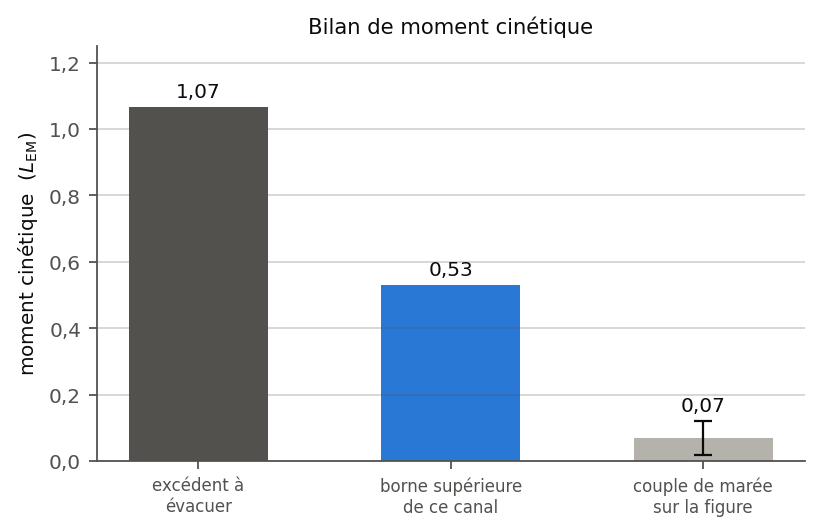
\includegraphics[width=0.62\textwidth]{fig_bilan_fr.png}
\caption{Excédent de moment cinétique à évacuer, borne supérieure du retrait par capture de matière, et couple de marée exercé sur la figure de la proto-Terre lors d'un passage unique (intervalle pour $k_2/Q$ entre $0{,}02$ et $0{,}10$).}
\label{fig:bilan}
\end{figure}

\paragraph{Bilan de masse.}
Au plus près du survol, la proto-Terre et le perturbateur constituent un couple transitoire dont les lobes de Roche mesurent respectivement $1{,}15$ et $1{,}12\,R_\oplus$ \cite{Eggleton1983} ; la proto-Terre remplit le sien à $148\,\%$, ce qui explique l'ampleur du soulèvement. La masse capturée est elle-même bornée par l'inventaire : $M_{\mathrm{cap,max}} \le \phi_{\oplus\to B}\,S_\oplus/\langle j_z\rangle_{\mathrm{lift}} \simeq 4{,}1\,M_L$, soit environ $5\,\%$ de la masse terrestre. La proto-Terre n'était donc, au plus, qu'environ $5\,\%$ plus massive avant la rencontre, ce qui s'accorde avec les scénarios d'accrétion tardive.

\paragraph{Réorientation de l'axe de rotation.}
Un passage incliné exerce un couple qui n'est pas aligné avec l'axe de rotation, et il est légitime de demander quelle réorientation il produit. Un élément de surface en corotation porte, au moment de son lâcher, $\mathbf{j} = \Omega_\oplus\,(\varpi^2\hat{\mathbf{z}} - z\,\mathbf{r}_\perp)$ : la composante transverse change de signe entre les deux hémisphères et tourne avec la longitude, de sorte qu'elle se compense en grande partie sur la population capturée. La somme pondérée par la masse, évaluée à la position réelle de chaque élément au moment de son lâcher, donne un vecteur emporté faisant $1{,}1^\circ$ avec l'axe de rotation à $i_B = 20^\circ$, $1{,}4^\circ$ à $25^\circ$ et $1{,}6^\circ$ à $30^\circ$. Rapporté au spin restant, le basculement de l'axe qui en résulte, $\Delta L_\perp / S_{\mathrm{post}}$, reste de l'ordre d'un demi-degré au plus, même lorsque le retrait atteint sa borne.

Ce résultat est négatif quant à l'origine de l'obliquité terrestre, que ce mécanisme n'explique pas, mais positif quant à sa compatibilité : le passage n'impose aucune réorientation incompatible avec l'état observé. La matière retombée, dont le moment cinétique a été modifié par $B$, et le couple exercé sur la figure aplatie de la proto-Terre ne sont pas traités ici et restent à évaluer séparément.

\section{Un contrôle négatif : ce canal ne fournit pas la masse lunaire}

Pour un passage rigoureusement coplanaire, la condition pour que la couche la plus externe franchisse la limite de Roche se réduit à :
\begin{equation}
\mathcal{L} = \tilde{\omega}\sqrt{a} + \frac{\sqrt{2}\,\mu_B}{\sqrt{1+\mu_B}} \cdot \frac{a^2}{b^{3/2}} \ge \sqrt{a_R/R_\oplus} = 1{,}704,
\end{equation}
avec $a = R_{\mathrm{eq}}/R_\oplus$ et $b = q_B/R_\oplus$, ce qui donne $\mathcal{L} = 1{,}800$ pour la configuration de référence. Cependant, le dégagement du disque impose un survol incliné ($i_B \gtrsim 20^\circ$). La composante tangentielle de la marée décroît en $\cos^2 i_B$, et le calcul direct confirme cette loi : le décile supérieur de la population liée tombe à $1{,}75$ à $20^\circ$, $1{,}68$ à $25^\circ$ et $1{,}60$ à $30^\circ$, sous le seuil critique de Roche de $1{,}704$ (figure~\ref{fig:controle}).

\noindent\textbf{Ce que cela exclut :} À l'inclinaison imposée par la géométrie, et dans la configuration de référence, aucun matériau soulevé de la bande de basses latitudes ne franchit directement la limite de Roche. Ce résultat ne dépend pas du profil de densité de la proto-Terre : si la couche la plus favorable n'atteint pas le seuil, aucune répartition de masse ne peut produire une masse lunaire par cette voie. Le soulèvement superficiel est donc, dans cette configuration, un vecteur d'alimentation du réservoir et d'évacuation du moment cinétique, et non un mécanisme de fabrication directe de la Lune. La masse lunaire provient principalement du réservoir circumterrestre secondaire préexistant, que le passage de $B$ réorganise et aide à étendre au-delà de Roche. La fenêtre se rouvre si la proto-Terre est plus dilatée : à $R_{\mathrm{eq}} = 1{,}80\,R_\oplus$, $2$ à $3\,\%$ de la matière soulevée franchit la limite à $25^\circ$, au prix d'une marge de non-contact ramenée de $7$ à $3\,\%$.

\begin{figure}[htbp]
\centering
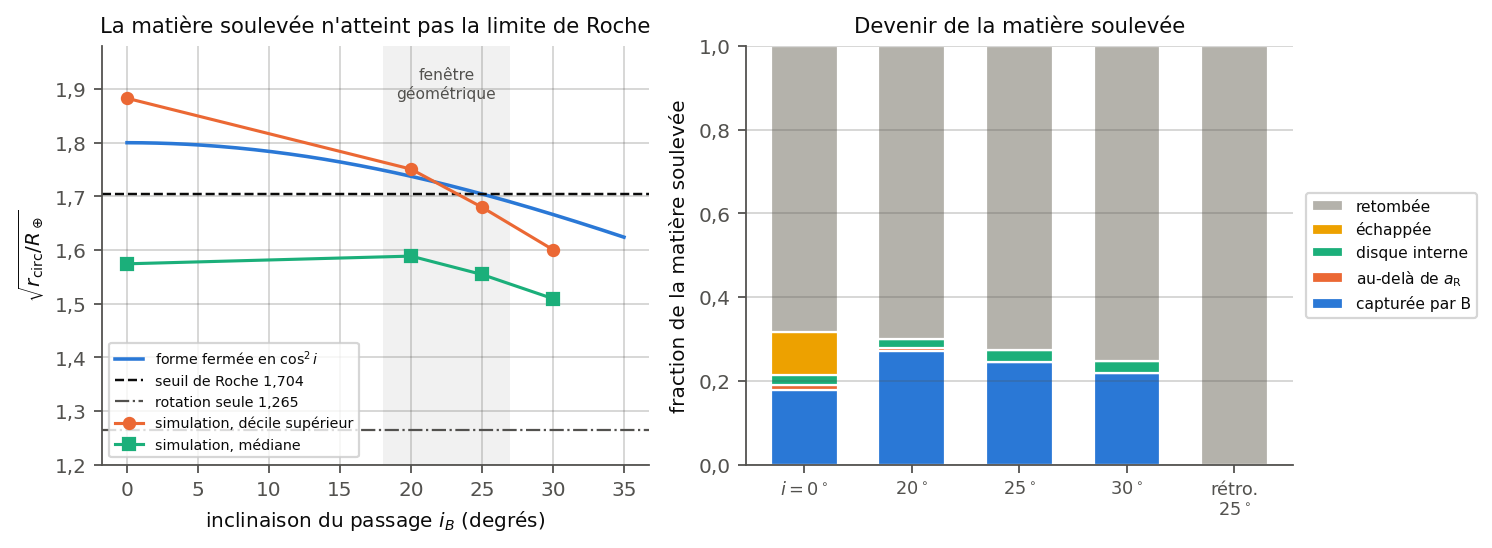
\includegraphics[width=\textwidth]{fig_controle_fr.png}
\caption{À gauche : $\sqrt{r_{\mathrm{circ}}/R_\oplus}$ de la population liée en fonction de l'inclinaison du passage, médiane et décile supérieur, comparés à la forme fermée coplanaire corrigée en $\cos^2 i$. La bande grisée est la fenêtre d'inclinaison imposée par le dégagement du disque. À droite : devenir de la matière soulevée pour chaque configuration, contrôle rétrograde compris.}
\label{fig:controle}
\end{figure}

\section{Ce que ce même passage rend disponible : les volatils}

Au périastre, pour $\rho_B = 3{,}93\,\mathrm{g\,cm^{-3}}$, le rayon de $B$ est de $1{,}10\,R_\oplus$ pour un lobe de Roche de $1{,}12\,R_\oplus$ (rempli à $98\,\%$). Une enveloppe volatile de seulement $146\,\mathrm{km}$ suffit pour déclencher un débordement.

Le flash thermique issu de l'océan magmatique ($3{,}4 \times 10^6\,\mathrm{W\,m^{-2}}$ à $3\,R_\oplus$) ne peut vaporiser un océan par simple enthalpie en six heures (l'énergie absorbée ne permet de sublimer que $\sim 4 \times 10^{18}\,\mathrm{kg}$, soit $0{,}003$ océan). Son rôle physique fondamental est de dilater l'échelle de hauteur atmosphérique :
\begin{equation}
H = \frac{k_B T}{\mu g},
\end{equation}
qui passe de $18\,\mathrm{km}$ à $300\,\mathrm{K}$ à $168\,\mathrm{km}$ à $2800\,\mathrm{K}$. Dilatée d'un ordre de grandeur, l'enveloppe atteint les points de Lagrange. La chaleur rend la matière expulsable ; le champ de marée l'expulse.

Les volatils évacués par le point de Lagrange extérieur s'échappent le long de la trajectoire hyperbolique de $B$, ensemençant une traînée héliocentrique de débris sur des orbites proches de celle de la Terre. Dans la théorie proposée, la ré-accrétion gravitationnelle séculaire de cette traînée s'étale sur plusieurs millions à plusieurs dizaines de millions d'années à mesure que l'océan magmatique terrestre refroidit, ce qui évite une livraison instantanée de l'eau à une Terre encore extrêmement chaude. La Terre constitue le puits principal de cette ressource volatile ; une fraction plus faible peut être interceptée par le réservoir circumterrestre et incorporée à la Lune au cours de sa relaxation et de son accrétion.

\paragraph{Minéralogie du perturbateur.} La condition de non-contact $q_B > R_{\mathrm{eq}} + R_B$ impose $\rho_B \gtrsim 2{,}4$--$3{,}9\,\mathrm{g\,cm^{-3}}$, désignant $B$ non comme un corps glacé, mais comme un corps silicaté différencié pourvu d'une enveloppe volatile, représentatif des grands planétésimaux hydratés formés au-delà de la ligne des glaces et perturbés vers l'intérieur. Son devenir héliocentrique ultérieur, qui n'exige pas qu'il subsiste dans le Système solaire actuel, relève du problème de l'instabilité orbitale primordiale \cite{Nesvorny2011}.

\paragraph{Réserves.} L'eau lunaire présente une composition isotopique de l'hydrogène proche de celle de l'eau terrestre et des chondrites carbonées \cite{Saal2008, Saal2013}, ce qui est cohérent avec une lignée commune tout en restant compatible avec d'autres voies d'apport. Deux contraintes demeurent hors du champ de cet article : la chronologie du mélange de cette eau dans le manteau, et le rapport D/H du perturbateur, qui deviendrait une contrainte forte sur sa région de formation.

\section{Limites et rétroaction dynamique}

Le présent travail intègre des particules-tests : il n'inclut ni pression, ni autogravité, ni collisions entre éléments arrachés, alors que la couche soulevée est un fluide. La masse absolue soulevée n'est pas calculée ; seule l'est la fraction de la bande qui quitte la surface, et sa conversion en masses lunaires exige un profil de densité des couches externes. C'est pourquoi le retrait de moment cinétique est donné ici sous forme de borne supérieure.

\paragraph{Rétroaction sur le spin.} La matière quittant le corps au voisinage du rayon équatorial emporte du moment cinétique et du moment d'inertie dans le même rapport, $j_z \simeq \Omega_\oplus R_{\mathrm{eq}}^2$, de sorte que la vitesse angulaire $\Omega_\oplus$ demeure inchangée au premier ordre : ce qui décroît est le moment cinétique total et le moment d'inertie, non la rotation. La porte de marée $2\mu_B (R_{\mathrm{eq}}/q_B)^3 + \tilde{\omega}^2 \ge 1$ ne se referme donc pas par ralentissement pendant le survol. La limitation véritable n'est pas temporelle mais comptable : c'est la borne d'inventaire établie plus haut. Les lâchers sont d'ailleurs fortement concentrés, $99{,}9\,\%$ d'entre eux se produisant dans une fenêtre de $\pm 2\,\mathrm{h}$, sur une étendue totale de $3{,}1\,\mathrm{h}$.

\paragraph{Bilan vectoriel.} Seul le vecteur emporté par la matière capturée est calculé. La matière retombée, dont le moment cinétique a été modifié par $B$, et le couple exercé sur la figure aplatie de la proto-Terre restent à intégrer. Des simulations hydrodynamiques dissipatives complètes (SPH) devront quantifier ces effets et fixer la valeur effective du retrait sous la borne.

\section{Ce qui réfuterait ce modèle}

Le mécanisme est définitivement invalidé, en tant que voie d'évacuation du moment cinétique, si :
\begin{enumerate}
    \item Une modélisation hydrodynamique dissipative complète (SPH) abaisse $\phi_{\oplus\to B}$ sous environ $0{,}10$, ramenant la borne de retrait sous $0{,}2\,L_{\mathrm{EM}}$ : ce canal deviendrait marginal devant la résonance d'évection.
    \item La masse effectivement soulevée pendant le survol, calculée avec un profil de densité réaliste des couches externes, ne porte qu'une fraction négligeable du spin du corps.
    \item Le bilan vectoriel complet, incluant la matière retombée et le couple sur la figure aplatie, impose une réorientation de l'axe incompatible avec l'obliquité observée de $23{,}4^\circ$.
    \item Les modèles thermochimiques démontrent que la traînée de volatils héliocentrique ne peut survivre à la photodissociation solaire sur l'échelle de temps de ré-accrétion séculaire.
\end{enumerate}

\paragraph{Disponibilité des données.} Le code d'intégration numérique (\texttt{stripping.py}, \texttt{analyse.py}) et le script qui reproduit l'ensemble des nombres et figures de cet article (\texttt{reproduire.py}) sont archivés avec la monographie compagne \cite{Debailleul2026} sur GitHub (\url{https://github.com/Orion4622/moon-and-water}).

\paragraph{Remerciements.} L'auteur est chercheur indépendant et accueillera avec intérêt toute critique constructive portant en particulier sur l'absence de traitement dissipatif de la couche fluide arrachée, la masse absolue soulevée et la généralisation vectorielle du bilan de moment cinétique.

\begin{thebibliography}{99}
\bibitem{Murray1999} C. D. Murray et S. F. Dermott, \emph{Solar System Dynamics}, Cambridge University Press, 1999.
\bibitem{Tremaine2009} S. Tremaine, J. Touma et F. Namouni, \og Satellite dynamics on the Laplace surface \fg, \emph{The Astronomical Journal}, 137 (2009), p.~3706--3717.
\bibitem{Cuk2012} M. \'{C}uk et S. T. Stewart, \og Making the Moon from a fast-spinning Earth: a giant impact followed by resonant despinning \fg, \emph{Science}, 338 (2012), p.~1047--1052.
\bibitem{Canup2023} R. M. Canup, K. Righter, N. Dauphas et al., \og Origin of the Moon \fg, \emph{Reviews in Mineralogy and Geochemistry}, 89 (2023), p.~53--102.
\bibitem{Pahlevan2015} K. Pahlevan et A. Morbidelli, \og Collisionless encounters and the origin of the lunar inclination \fg, \emph{Nature}, 527 (2015), p.~492--494.
\bibitem{Eggleton1983} P. P. Eggleton, \og Approximations to the radii of Roche lobes \fg, \emph{The Astrophysical Journal}, 268 (1983), p.~368--369.
\bibitem{Ida1997} S. Ida, R. M. Canup et G. R. Stewart, \og Lunar accretion from an impact-generated disk \fg, \emph{Nature}, 389 (1997), p.~353--357.
\bibitem{Salmon2012} J. Salmon et R. M. Canup, \og Lunar accretion from a Roche-interior fluid disk \fg, \emph{The Astrophysical Journal}, 760 (2012), p.~83.
\bibitem{Kokubo2000} E. Kokubo, S. Ida et J. Makino, \og Evolution of a circumterrestrial disk and formation of a single moon \fg, \emph{Icarus}, 148 (2000), p.~419--436.
\bibitem{Saal2008} A. E. Saal et al., \og Volatile content of lunar volcanic glasses and the presence of water in the Moon's interior \fg, \emph{Nature}, 454 (2008), p.~192--195.
\bibitem{Saal2013} A. E. Saal, E. H. Hauri, J. A. Van Orman et M. J. Rutherford, \og Hydrogen isotopes in lunar volcanic glasses and melt inclusions reveal a carbonaceous chondrite heritage \fg, \emph{Science}, 340 (2013), p.~1317--1320.
\bibitem{Nesvorny2011} D. Nesvorn\'y, \og Young Solar System's fifth giant planet? \fg, \emph{The Astrophysical Journal Letters}, 742 (2011), L22.
\bibitem{Debailleul2026} M. Debailleul, \emph{The Moon and Water: Secondary Circumterrestrial Disk and Non-Collisional Passage of a Planetary Body}, Zenodo, 2026. doi:\href{https://doi.org/10.5281/zenodo.22770198}{10.5281/zenodo.22770198}.
\end{thebibliography}

\end{document}
